---
title: Pos 圏の射影的対象と選択公理
author: 石井大海
description: 「Pos圏における射影的対象のなす充満部分圏が集合圏と同型である」ことと選択公理の同値性の証明。
tag: 圏論,集合論,選択公理,ロジック,数理論理学,数学基礎論
date: 2012/03/02 23:17:00 JST
latexmk: -pdflua
---
\RequirePackage{luatex85}
\documentclass[a4j]{ltjsarticle}
\usepackage[hiragino-pron]{luatexja-preset}
\usepackage{mystyle}
\usepackage{luatexja-otf}
\usepackage{dsfont}
\DeclareMathAlphabet{\mathrsfs}{U}{rsfso}{m}{n}
\renewcommand{\mathscr}[1]{\mathup{\mathrsfs{#1}}}
\usepackage{fixme}
\usepackage[super]{nth}
\usepackage[bookmarksnumbered,pdfproducer={LuaLaTeX},%
            luatex,psdextra,pdfusetitle,pdfencoding=auto]{hyperref}
\usepackage[backend=biber, style=math-numeric]{biblatex}
\addbibresource{myreference.bib}
\renewcommand{\emph}[1]{\textgt{\textsf{#1}}}
\usetikzlibrary{shapes,shapes.geometric,positioning,math,fpu}
\tikzset{
 node distance=2cm, auto,
 column sep=1.5cm, row sep = 1.5cm,
 description/.style={fill=white,inner sep=1.5pt,auto=false}}

%% その他記号
\newcommand{\dis}{\mathrm{dis}}
\newcommand{\Pos}{\mathbf{Pos}}

\title{$\Pos$の射影的対象と選択公理}
\author{石井大海}

\begin{document}
\maketitle
\section{概要}
Awodey~\cite{Awodey:2010}の演習問題を解いていたところ,選択公理と同値な
命題を見付けたので証明を試みました.手許の文献でこの同値性に言及している
ものはなかったと思います.
\section{準備}
以下では,圏$\Pos$とは,半順序集合(partially ordered set,以下poset)を
対象,その間の単調写像を射とした圏であるとします.
恒等写像は明らかに単調ですし,単調写像と単調写像の合成が再び単調となるこ
とからこれは実際に圏となります.

\begin{definition}[射影的]
 圏${\bf C}$の対象$P$が{\bfseries 射影的}(projective)であるとは,任意の
 対象$E, X \in {\bf C}$と射$f: P \to X$およびエピ射$e: E \epi X$が与えら
 れたとき,次の図式を可換にする(一意とは限らない)射$\hat{f}: P \to E$
 が必ず存在することである.

 \begin{center}
   \begin{tikzpicture}
   \node (P) {$P$};
   \node (X) [right of=P] {$X$};
   \node (E) [above of=X] {$E$};
   \draw[->] (P) to node [swap] {$f$} (X);
   \draw[->>] (E) to node {$e$} (X);
   \draw[->, dashed] (P) to node {$\hat{f}$} (E);
  \end{tikzpicture}
 \end{center}
\end{definition}

射影的対象の概念を用いて,選択公理を言い換えたものが以下です.
\begin{theorem}\label{projective}
 以下の命題は選択公理と同値.
 \begin{quotation}
  圏$\Sets$ の任意の対象は射影的である.
 \end{quotation}
\end{theorem}
\begin{proof}
 @alg-d さんのサイト\cite{alg-d}を参照.
\end{proof}

\begin{theorem}\label{epi and surj}
 圏$\Pos$のエピ射は全射単調写像と完全に一致する.
\end{theorem}
\begin{proof}[概略]
 $e$がエピ射でないとすると,$he = h'e$ かつ $h \neq h'$なる射が存在し,
 $e$の定義域の外に$h(x) \neq h'(x)$なる$x$が存在することになり全射となら
 ない.また,エピ射かつ全射でない単調写像$e$が存在したとすると,$e$ の定義域の
 外から一点を取り,その行き先を上手く違えた $h, h'$ を取ってやることで矛
 盾を導くことが出来る.
\end{proof}

また,以下では次の事実を用いる.
\begin{fact}
 通常の集合$S$は,離散poset,即ち,各元$x \in S$についての反射律のみ
 を仮定して得られる poset と見做すことで $\Pos$ の対象と見做すことが出来る.
\end{fact}

\section{$\Pos$と$\Sets$の関係}
\begin{theorem}
 以下の命題は選択公理と同値.
 \begin{quotation}
  集合を離散 poset と見做すことによって,$\Sets$ は $\Pos$ の射影的対象
  からなる充満部分圏となる.
 \end{quotation}
\end{theorem}
\begin{proof}
 \begin{enumerate}
  \item \underline{\bfseries 必要性.}

	集合の間の写像は,対応する離散 poset の間の単調写像と見做すこと
	が出来るので,結局は$\Pos$の射影的対象と離散posetが一致すること
	を示せばよい.

	まず,任意の集合$S$は$\Pos$で射影的であることを示そう.$S$を集合,
	即ち離散poset,$E, X$を任意のposetとし,単調写像$f: S \to X$およ
	びエピ射$e: E \epi X$が与えらえているとする.
	今,poset $A$ に対応する台集合を$|A|$,単調写像$f$の台写像を
	$|f|$で表わすことにすると,定理\ref{epi and surj}より$\Pos$での
	エピ射は全射でもあることに注意すると,$\Sets$で次の図式を可換に
	する射$\hat{f}: |S| \to |E|$が存在する.

        \begin{center}
 	 \begin{tikzpicture}
	  \node (S) {$|S|$};
	  \node (X) [right of=P] {$|X|$};
	  \node (E) [above of=X] {$|E|$};
	  \draw[->] (S) to node [swap] {$|f|$} (X);
	  \draw[->>] (E) to node {$|e|$} (X);
	  \draw[->, dashed] (S) to node {$|\hat{f}|$} (E);
	 \end{tikzpicture}
        \end{center}

	あとは,$|\hat{f}|$が単調写像となっていることを示せばよい.$S$は
	離散posetより,成立する順序関係は反射律のみであるので,特に
	$|\hat{f}|(a) \leq |\hat{f}|(a)$が云えればよい.しかるに,$E$は
	posetであったので反射律が成立し,特に$|\hat{f}|(a) \leq
	|\hat{f}|(a)$ が常に成立している.よって$|\hat{f}|$は単調写像.
	よって状況を$\Pos$に引き戻して
        \begin{center}
 	 \begin{tikzpicture}
	  \node (S) {$S$};
	  \node (X) [right of=P] {$X$};
	  \node (E) [above of=X] {$E$};
	  \draw[->] (S) to node [swap] {$f$} (X);
	  \draw[->>] (E) to node {$e$} (X);
	  \draw[->] (S) to node {$\hat{f}$} (E);
	 \end{tikzpicture}
        \end{center}
	が可換となる.よって任意の集合は$\Pos$で射影的である.

	逆に,$P \in \Pos$を射影的対象とする.$P$の元からなる離散posetを
	$\dis(P)$と書くことにする.写像 $i:\dis(P) \epi P$ を
	$i(a) = a$で定めると,これはは明らかに全射単調写
	像であり,従って$\Pos$のエピ射である.よって,以下を可換にするよ
	うな $\hat{1}_P: P \to \dis(P)$が存在する.
        \begin{center}
 	 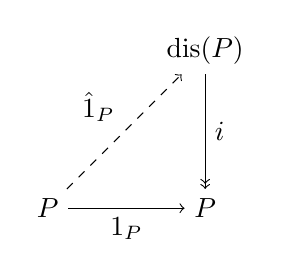
\begin{tikzpicture}
	  \node (P) {$P$};
	  \node (P') [right of=P] {$P$};
	  \node (disP) [above of=P'] {$\dis(P)$};
	  \draw[->] (P) to node [swap] {$1_P$} (P');
	  \draw[->>] (disP) to node {$i$} (P');
	  \draw[->,dashed] (P) to node {$\hat{1}_P$} (disP);
	 \end{tikzpicture}
        \end{center}	
すなわち,$i \circ \hat{1}_P = 1_P$である.特に$|P| = |\dis(P)|$
	であり,定義から$|i| = 1_{|P|} = 1_{|\dis(P)|}$となる.すると,
	\begin{align*}
	 | \hat{1}_P \circ i | &= |\hat{1}_P| \circ |i|
	                        = |\hat{1}_P| \circ 1_{|P|}
	                        = |\hat{1}_P|\\
	                       &= 1_{|P|} \circ |\hat{1}_P|
	                        = |i| \circ |\hat{1}_P|
	                        = |i \circ \hat{1}_P| \\ &= |1_P|
	                        = 1_{|P|} = 1_{|\dis(P)|} = |1_{\dis(P)}|\\
	 \therefore \hat{1}_P \circ i &= 1_{\dis(P)}\;\;\text{in}\ \Pos
	\end{align*}
	よって,$\hat{1}_P$は$\Pos$での同型射となる.今,$\dis(P)$は離散
	poset だったので,それと同型となる$P$もまた離散posetとなる.

	以上より示された.
  \item \underline{\bfseries 十分性.}

	$\Pos$の射影的対象と離散posetが一致すると仮定する.今,Factより
	任意の集合$A$は離散posetと同一視出来る.すると,A は$\Pos$で射影
	的であり.他の集合$E, X$も$\Pos$の対象と見做せ,その間の全射
	$e: E \to X$と写像$f: A \to X$が存在すれば,それらはposetとして
	の$A, E, X$間の単調写像と同一視出来,とくに$e$は$\Pos$でエピ射と
	なる.すると,それらに対して下の図式を可換にする$\hat{f}:A\to E$
	が存在する.
        \begin{center}
 	 \begin{tikzpicture}
	  \matrix (m) [matrix of math nodes] { & E \\ A & X \\};
	  \draw[->] (m-2-1) to node [swap] {$f$} (m-2-2);
	  \draw[->>] (m-1-2) to node {$e$} (m-2-2);
	  \draw[->, dashed] (m-2-1) to node {$\hat{f}$}(m-1-2);
	 \end{tikzpicture}
        \end{center}	
再び$\Sets$に戻って考えれば,これは任意の集合は射影的であると云
	うことであり,定理\ref{projective}より選択公理が従う.
 \end{enumerate}
\end{proof}

\printbibliography[title=参考文献]
\end{document}
